\documentclass[french]{article}
\usepackage[T1]{fontenc}
\usepackage[latin9]{inputenc}
\usepackage{geometry}
\geometry{verbose,tmargin=2cm,bmargin=2.5cm,lmargin=2.5cm,rmargin=3cm}
\usepackage{amsmath}
\usepackage{amssymb}
\usepackage{graphicx}

\makeatletter

\newcommand{\noun}[1]{\textsc{#1}}


\renewcommand{\descriptionlabel}[1]{\hspace\labelsep\upshape\bfseries #1:}
\renewenvironment{description}{\list{}{%
  \setlength{\itemsep}{-2pt}
  \advance\leftmargini6\p@ \itemindent-12\p@
  \labelwidth\z@ \let\makelabel\descriptionlabel}%
}{
  \endlist
}

\usepackage{xcolor}
\usepackage{fancyhdr}

\definecolor{INSA_GM}{cmyk}{0.6,0,0,0}
\definecolor{INSA_GRIS}{cmyk}{0.7,0.6,0.5,0.3}
\definecolor{INSA_BLEU}{cmyk}{1,0.9,0.1,0}

\newcommand{\insertrefproj}[1]{}
\newcommand{\refproj}[1]{\renewcommand{\insertrefproj}{\textbf{\color{INSA_GRIS}#1}}}

\fancypagestyle{courant}{
\fancyhf{}
    \setlength{\headheight}{27pt}
    \fancyhead[L]{\raisebox{-2mm}{\includegraphics[width=30mm]{image/logoINSA.jpg}}}
\fancyhead[C]{}
\fancyhead[R]{\color{INSA_GRIS}\thepage}
\fancyfoot[L]{\insertrefproj}
\fancyfoot[R]{}
\renewcommand{\headrulewidth}{0pt}
\renewcommand{\footrulewidth}{0.2pt}
}

\fancypagestyle{special}{
  \pagestyle{courant}
  \fancyfoot{}
\renewcommand{\footrulewidth}{0pt}
}

\fancypagestyle{plain}{
  \fancyhf{}
  \pagestyle{courant}
}
\title{Projet GM3}
\refproj{GM3/MIPP/2022 - 23}

\pagestyle{plain}

\makeatother

\usepackage{babel}
\makeatletter
\addto\extrasfrench{%
   \providecommand{\og}{\leavevmode\flqq~}%
   \providecommand{\fg}{\ifdim\lastskip>\z@\unskip\fi~\frqq}%
}

\makeatother
\usepackage{listings}
\renewcommand{\lstlistingname}{Listing}

\begin{document}
\thispagestyle{empty}

\begin{minipage}[c]{0.4\textwidth}%
\includegraphics[width=1\textwidth]{../../MIPP/lyx/IMAGE/logoINSA}%
\end{minipage}\hfill{}%
\begin{minipage}[c]{0.4\textwidth}%
\centering \textcolor{INSA_GM}{\textbf{\Large{}Projet MMSN }\\
\textbf{\Large{}GM3 2022 - 2023}}%
\end{minipage}\vspace{7cm}

\noindent\begin{minipage}[c]{1\textwidth}%
\centering\textcolor{INSA_BLEU}{\textbf{\Huge{}Gradient Conjugué
}}%
\end{minipage}\vfill{}
\vfill{}

\begin{minipage}[t]{6cm}%
\large \textcolor{INSA_GRIS}{ \textbf{Étudiants :} \\
LANGOLFF Clément\\
KESSLER Aymeric}%
\end{minipage}\hfill{}%
\begin{minipage}[t]{9cm}%
\large \textcolor{INSA_GRIS}{\textbf{Enseignant-responsable du projet
:}\\
 \noun{El Bouchairi Imad} }%
\end{minipage}\vspace{2cm}

\newpage{}

\tableofcontents{}

\newpage{}

\part{Introduction}

\subsection{Fonctionnelle à minimiser}

La méthode du gradient conjugué fait partie des méthodes de descente.
À chaque itération, on determine un vecteur direction $d_{k}$ et
un scalaire $\alpha_{k}$ permettant de calculer une nouvelle approche
de la solution $x_{k+1}=x_{k}+\alpha_{k}d_{k}$. L'objectif des méthodes
de descente est de minimiser la fonctionnelle\nocite{Lascaux2004-gj}
:

\begin{equation}
J(x)=\frac{1}{2}(Ax|x)-(b|x)=\frac{1}{2}x^{T}Ax-x^{T}b
\end{equation}
 où $A$ est une matrice symétrique définit positive ( $A^{T}=A$
et $(Ax|x)>0\lor x\neq0$). Dans ce cas, J est aussi définit positive
et est quadratique. 

Trouver le minimum de la fonctionnelle J revient à trouver la solution
du système $Ax=b$. \\
En effet, comme J est quadratique est positive, J est connexe et son
minimum unique $\overline{x}$ est obtenu en annulant le gradient
de J : $\nabla J(\overline{x})=A\overline{x}-b=0$ $\iff\overline{x}$
solution du système.\\
\\
\\
On note $r(x)=b-Ax=A(\overline{x}-x)$ le résidu du système et $e(x)=x-\overline{x}$
l'erreur ou la différence entre la solution calculée et la solution
exacte. Minimiser $J$ est équivalant à minimiser la fonctionnelle
$E$ définit par
\begin{equation}
E(x)=(A(x-\overline{x})|x-\overline{x})=(Ae(x)|e(x))
\end{equation}

En effet, $E(x)=2J(x)+\underbrace{(A\overline{x}|\overline{x})}_{cst>0}$.
\\
\\

Comme $A$ est symétrique définit positive, $(Ax,y)=(x,Ay)$ définit
un produit scalaire et $E(x)=(Ae(x)|e(x))=\parallel e(x)\parallel_{A}{{}^2}$
où $\parallel e(x)\parallel_{A}$ est la norme associée à ce produit
scalaire. Dans la suite, nous utiliserons la fonctionnelle $E$ pour
trouver la solution du système $Ax=b$.

\subsection{Choix optimal de $\alpha_{k}$ pour une direction fixée $d_{k}$}

On suppose que la direction $d_{k}$ est fixée. L'objectif est de
minimiser la fonctionnelle $E(x_{k})$ à chaque itération. Or
\begin{align*}
E(x_{k+1}) & =E(x_{k}+\alpha_{k}d_{k})=(A(x_{k}+\alpha_{k}d_{k}-\overline{x})|x_{k}+\alpha_{k}d_{k}-\overline{x})\\
 & =E(x_{k})-2\alpha_{k}(r_{k}|d_{k})+\alpha_{k}{{}^2}(Ad_{k}|d_{k})
\end{align*}

qui est un polynôme de degrés 2 en $\alpha_{k}$ et atteint son minimum
en $\frac{-b}{2a}=\frac{(r_{k}|d_{k})}{(Ad_{k}|d_{k})}$.

Ainsi, peut importe la direction $d_{k}$ choisie, le minimum de $E$
sera atteint pour 
\begin{equation}
\alpha_{opt}=\frac{(r_{k}|d_{k})}{(Ad_{k}|d_{k})}
\end{equation}
.

De plus, on a 
\begin{equation}
r_{k+1}=b-Ax_{k+1}=r_{k}-\alpha_{k}Ad_{k}
\end{equation}

et le résidu obtenu à l'itération $k$ est orthogonale à la direction
$d_{k}$: 
\begin{align}
(r_{k+1}|d_{k}) & =(r_{k}-\alpha_{k}Ad_{k}|d_{k})\nonumber \\
 & =(r_{k}|d_{k})-\alpha_{k}(Ad_{k}|d_{k})\nonumber \\
 & =(r_{k}|d_{k})-\frac{(r_{k}|d_{k})}{(Ad_{k}|d_{k})}(Ad_{k}|d_{k})\\
 & =0\nonumber 
\end{align}
. 

\subsection{Choix de la direction optimal pour $\alpha_{opt}$}

Pour ce $\alpha_{opt}$, on a 
\begin{align*}
E(x_{k+1}) & =E(x_{k})-2\alpha_{k}(r_{k}|d_{k})+\alpha_{k}{{}^2}(Ad_{k}|d_{k})\\
 & =E(x_{k})-2\frac{(r_{k}|d_{k})}{(Ad_{k}|d_{k})}(r_{k}|d_{k})+\frac{(r_{k}|d_{k}){{}^2}}{(Ad_{k}|d_{k}){{}^2}}(Ad_{k}|d_{k})\\
 & =E(x_{k})-\frac{(r_{k}|d_{k}){{}^2}}{(Ad_{k}|d_{k})}\\
 & =E(x_{k})(1-\frac{(r_{k}|d_{k}){{}^2}}{E(x_{k})(Ad_{k}|d_{k})})
\end{align*}

Or $E(x_{k})=(Ae(x_{k})|e(x_{k}))$ et $r_{k}=A(x_{k}-\overline{x})=-Ae(x_{k})$$\iff e(x_{k})=-A^{-1}r_{k}$.
\\
Ainsi $E(x_{k})=(A^{-1}r_{k}|r_{k})$.\\
\\

Donc 
\begin{equation}
E(x_{k+1})=E(x_{k})(1-\frac{(r_{k}|d_{k}){{}^2}}{(A^{-1}r_{k}|r_{k})(Ad_{k}|d_{k})})
\end{equation}

Mais $E(x)$ est une fonctionnelle minimisante qui s'approche le plus
possible de la solution exacte $\overline{x}$, autrement dit on doit
avoir $E(x_{k+1})<E(x_{k})$ et $\underset{k\rightarrow+\infty}{lim}E(x_{k})=0$.

On pose $(u_{k})_{k\in\mathbb{N}}$ la suite définit par $u_{k}=$$1-\frac{(r_{k}|d_{k}){{}^2}}{(A^{-1}r_{k}|r_{k})(Ad_{k}|d_{k})}$.
On a 
\begin{align*}
E(x_{k+1}) & <E(x_{k})u_{k}\\
E(x_{k+1}) & <u_{k}^{k+1}E(x_{0})
\end{align*}

Donc $E(x_{k})$ définit une suite géométrique et converge si et seulement
si à partir d'un certain rang $k$, $|u_{k}|=|1-\frac{(r_{k}|d_{k}){{}^2}}{(A^{-1}r_{k}|r_{k})(Ad_{k}|d_{k})}|<1$.
Autrement dit, s'il existe une constante $\mu\in]0,1[$ tel que $\frac{(r_{k}|d_{k}){{}^2}}{(A^{-1}r_{k}|r_{k})(Ad_{k}|d_{k})}\geq\mu$.

Or $(Ad_{k}|d_{k})\leq\lambda_{1}||d_{k}||_{2}{{}^2}$ où $\lambda_{1}$
est la plus petite valeur propre de A. Et $(A^{-1}r_{k}|r_{k})\leq\frac{1}{\lambda_{n}}||r_{k}||_{2}{{}^2}$
où $\lambda_{n}$ est la plus grande valeur propre de A. Donc 
\[
\frac{(r_{k}|d_{k}){{}^2}}{(A^{-1}r_{k}|r_{k})(Ad_{k}|d_{k})}\geq\frac{\lambda_{1}}{\lambda_{n}}\frac{(r_{k}|d_{k}){{}^2}}{||d_{k}||_{2}{{}^2}||r_{k}||_{2}{{}^2}}=\underbrace{\frac{1}{cond_{2}(A)}}_{\in]0,1[}\underbrace{(\frac{r_{k}}{||r_{k}||_{2}}|\frac{d_{k}}{||d_{k}||_{2}}){{}^2}}_{\in[0,1]}
\]

Remarquons que $E(x_{k})_{k}$converge de plus en plus vite si $u_{k}$
est proche de 0, c'est a dire si $\mu$ est le plus proche possible
de 1. Ainsi, en choisissant une direction colinéaire au résidu $r_{k}$,
on a 
\[
E(x_{k+1})<(\underbrace{1-\frac{1}{cond_{2}(A)}}_{\in]0,1[})^{k}E(x_{0})
\]

On a donc toujours une convergence de la suite $E(x_{k})$ et le conditionnement
de la matrice A a une influence sur cette vitesse de convergence.
Plus le conditionnement est petit, plus la convergence est rapide.

On a vu que $\nabla J=-r$ donc le gradient est colinéaire au résidu
( remarque $\nabla E=-2r$ aussi colinéaire au résidu ).

\newpage{}

\part{Motivation du gradient conjugué}

\subsection{Analyse par méthode de projection}

D'après le paragraphe d'avant, plus le conditionnement de la matrice
est grand, plus la vitesse de convergence est faible. On souhaite
donc maximiser $\frac{(r_{k}|d_{k}){{}^2}}{(A^{-1}r_{k}|r_{k})(Ad_{k}|d_{k})}$
peu importe le conditionnement de la matrice $A$. L'idée est de faire
une combinaison linéaire du résidu et de la direction précédente pour
trouver la direction qui se rapproche le plus du centre (la solution
du système). la nouvelle direction se trouvera dans le plan généré
par $d_{k-1}$et $r_{k}$. On pose 
\begin{equation}
d_{k}=r_{k}+\beta_{k}d_{k-1}
\end{equation}
.

Comme $(r_{k+1}|d_{k})=0$ , on a 
\begin{align*}
\frac{(r_{k}|d_{k}){{}^2}}{(A^{-1}r_{k}|r_{k})(Ad_{k}|d_{k})} & =\frac{(r_{k}|r_{k}+\beta_{k}d_{k-1}){{}^2}}{(A^{-1}r_{k}|r_{k})(Ad_{k}|d_{k})}\\
 & =\frac{((r_{k}|r_{k})+\beta_{k}(r_{k}|d_{k-1})){{}^2}}{(A^{-1}r_{k}|r_{k})(Ad_{k}|d_{k})}\\
 & =\frac{(r_{k}|r_{k}){{}^2}}{(A^{-1}r_{k}|r_{k})(Ad_{k}|d_{k})}
\end{align*}

Ainsi maximiser $\frac{(r_{k}|d_{k}){{}^2}}{(A^{-1}r_{k}|r_{k})(Ad_{k}|d_{k})}$
revient à minimiser $(Ad_{k}|d_{k})$.

\begin{align*}
(Ad_{k}|d_{k}) & =(A(r_{k}+\beta_{k}d_{k-1})|r_{k}+\beta_{k}d_{k-1})\\
 & =\beta_{k}{{}^2}(Ad_{k-1}|d_{k-1})+2\beta_{k}(Ad_{k-1}|r_{k})+(Ar_{k}|r_{k})
\end{align*}

trinôme en $\beta_{k}$ dont le coefficient sur le degrés principale
est positif, le minimum est atteint en $\frac{-b}{2a}=-\frac{(Ad_{k-1}|r_{k})}{(Ad_{k-1}|d_{k-1})}$.

Ainsi la direction maximisant la vitesse de convergence est obtenue
pour 
\begin{equation}
\beta_{k}=-\frac{(Ad_{k-1}|r_{k})}{(Ad_{k-1}|d_{k-1})}
\end{equation}

De plus, on a 
\begin{align}
(Ad_{k-1}|d_{k}) & =(Ad_{k-1}|r_{k}+\beta_{k}d_{k-1})\nonumber \\
 & =(Ad_{k-1}|r_{k})-\frac{(Ad_{k-1}|r_{k})}{(Ad_{k-1}|d_{k-1})}(Ad_{k-1}|d_{k-1})\\
 & =0\nonumber 
\end{align}
 On dit que les directions choisies à chaque itération sont A-conjugués. 

Et 
\begin{align}
(r_{k}|d_{k}) & =(r_{k}|r_{k}+\beta_{k}d_{k-1})\nonumber \\
 & =(r_{k}|r_{k})+\beta_{k}\underbrace{(r_{k}|d_{k-1})}_{0}\\
 & =(r_{k}|r_{k})\nonumber 
\end{align}

On peut récrire $\beta_{k}$ en fonction du résidu :

on sait que $r_{k+1}=r_{k}-\alpha_{k}Ad_{k}$ donc $Ad_{k-1}=\frac{1}{\alpha_{k-1}}(r_{k-1}-r_{k})$

et comme 
\begin{align}
(r_{k+1}|r_{k}) & =(r_{k}-\alpha_{k}Ad_{k}|r_{k})\nonumber \\
 & =(r_{k}|r_{k})-\alpha_{k}(Ad_{k},r_{k})\nonumber \\
 & =(r_{k}|r_{k})-\alpha_{k}(Ad_{k},d_{k}-\beta_{k}d_{k-1})\nonumber \\
 & =(r_{k}|r_{k})-\alpha_{k}(Ad_{k},d_{k})+\alpha_{k}\beta_{k}\underbrace{(Ad_{k}|d_{k-1})}_{0}\\
 & =(r_{k}|r_{k})-\frac{(r_{k}|d_{k})}{(Ad_{k}|d_{k})}(Ad_{k},d_{k})\nonumber \\
 & =0\nonumber 
\end{align}

Donc

\begin{align}
\beta_{k} & =-\frac{(\frac{1}{\alpha_{k-1}}(r_{k-1}-r_{k})|r_{k})}{(\frac{1}{\alpha_{k-1}}(r_{k-1}-r_{k})|d_{k-1})}\nonumber \\
 & =-\frac{\overbrace{(r_{k-1}|r_{k})}^{0}-(r_{k}|r_{k})}{(r_{k-1}|d_{k-1})-\underbrace{(r_{k}|d_{k-1})}_{0}}\\
 & =\frac{(r_{k}|r_{k})}{(r_{k-1}|d_{k-1})}\nonumber \\
 & =\frac{(r_{k}|r_{k})}{(r_{k-1}|r_{k-1})}\nonumber 
\end{align}


\subsection{Algorithme pour la méthode du gradient conjugué}

\begin{lstlisting}
Fonction GradConj (Nmax,tol,A,x,r0)
	d = r0
	normeR0 = (r0,r0)
	TANT QUE normeR0 < tol FAIRE
		Ad = A*d
		alpha = normeR0 / (Ad,d)
		x = x + alpha * d
		r1 = r0 - alpha * Ad
		normeR1 = (r1,r1)
		beta = normeR1 / normeR0
		d = r1 + beta * d 
\end{lstlisting}
\newpage{}

\part{Applications}

\subsection{Étude en dimension 2}

En dimension 2, la fonction bilinéaire symétrique définit par la matrice
A est une paraboloïde et les lignes de niveau sont des ellipses. En
dimension 2, l'algorithme du gradient conjugué doit converger en seulement
2 itérations peu importe le conditionnement de la matrice. A l'inverse,
si le conditionnement de la matrice est mauvais, l'algorithme du gradient
descente a une vitesse de convergence très mauvaise. On peut interpréter
cette mauvaise convergence en observant des \og sauts de puce\fg{}
entre les courbes de niveau de la fonction. En effet, si la matrice
est mal conditionnée, ces ellipses sont très allongées ce qui implique
un déplacement très petit puisque la direction de descente est choisie
orthogonale à la ligne de niveau.

Considérons la matrice A =\begin{math}\displaystyle \left(\begin{array}{rr} \ 2 & -1 \\ -1 & 2 \end{array}\right)\end{math}
et b = \begin{math}\displaystyle \left(\begin{array}{rr} \ 1 \\ 1 \end{array}\right)\end{math} 

Conditionnement de A = 2.99999

\noindent\begin{minipage}[t]{1\columnwidth}%
\center

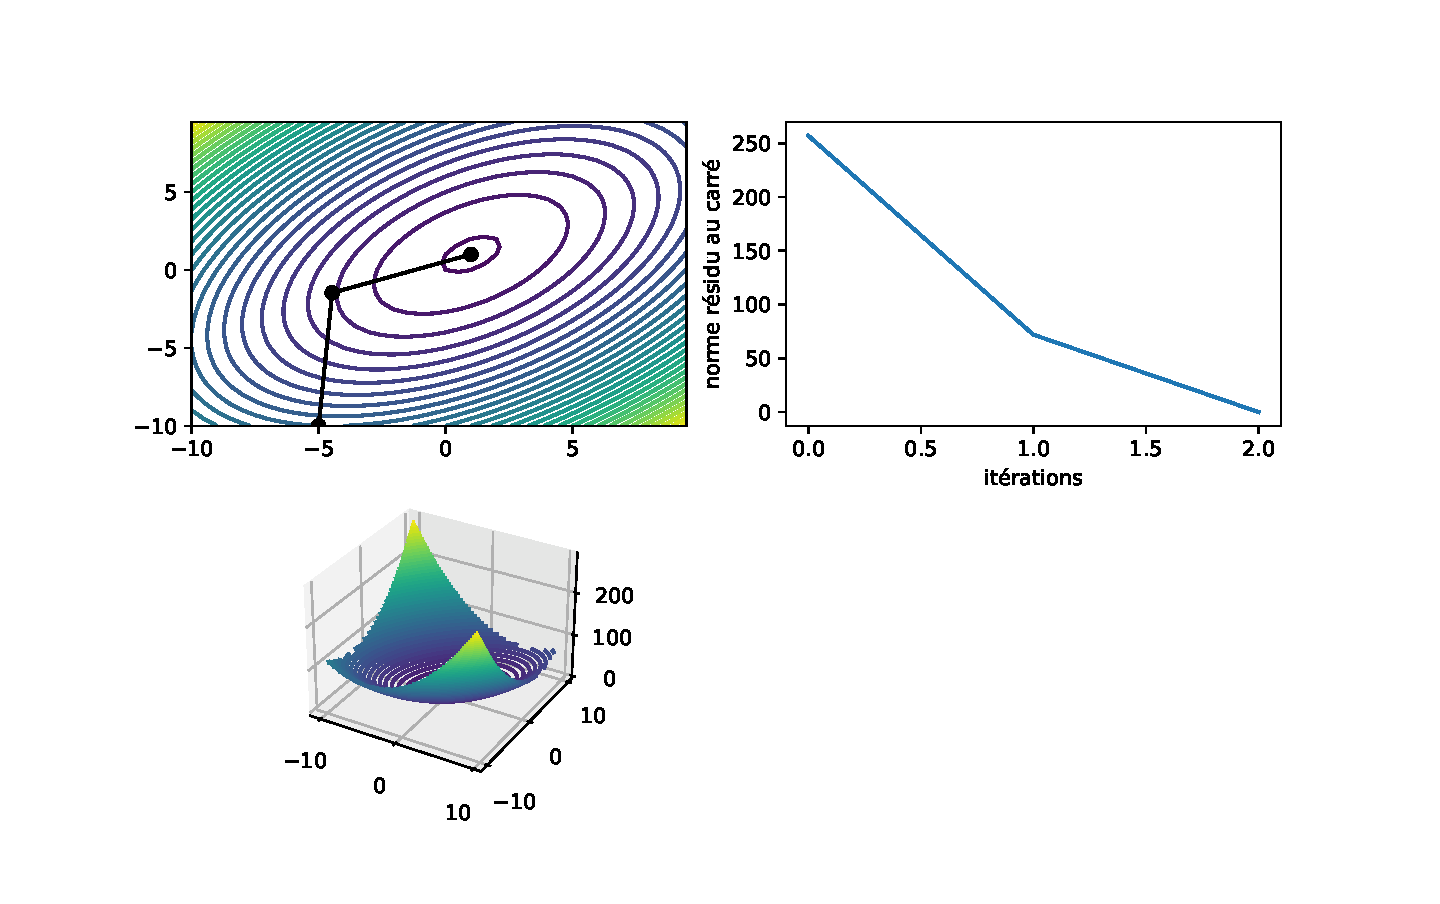
\includegraphics[scale=0.8]{image/gradientconj}

Algorithme du gradient conjugué appliqué à la matrice A pour $x_{0}=(-5,-10)$%
\end{minipage}

\noindent\begin{minipage}[t]{1\columnwidth}%
\center

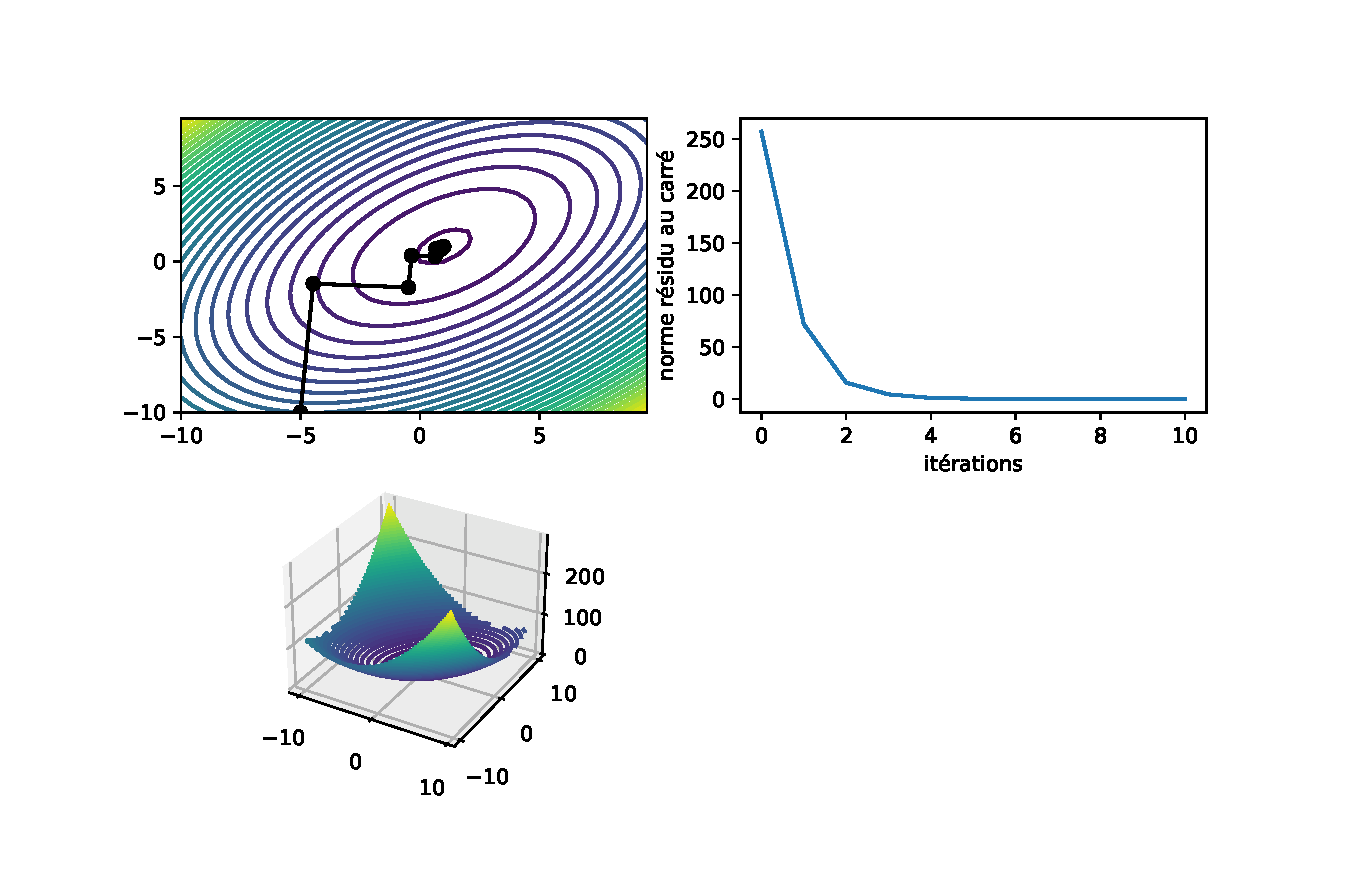
\includegraphics[scale=0.8]{image/descente}

Algorithme du gradient descente appliqué à la matrice A pour $x_{0}=(-5,-10)$%
\end{minipage}

\subsection{Application en dimension N}

On se place maintenant dans le cas infini A = \begin{math}\displaystyle \begin{pmatrix} 2 & -1 & 0 & \cdots & 0 \\ -1 & 2 & -1 & \ddots & \vdots \\ 0 & -1 & \ddots & \ddots & 0 \\ \vdots & \ddots & \ddots & 2 & -1 \\ 0 & \cdots & 0 & -1 & 2\end{pmatrix}\end{math}

Conditionnement de A = 16373

\noindent\begin{minipage}[t]{1\columnwidth}%
\center

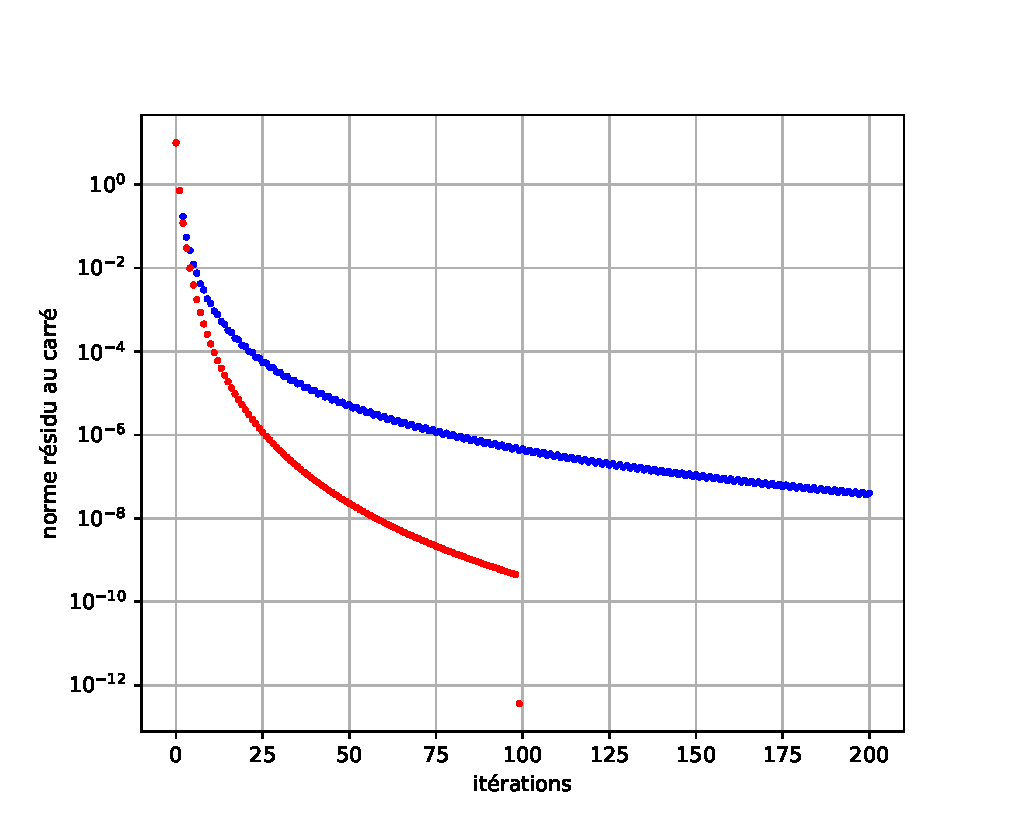
\includegraphics[scale=0.8]{image/comparaisonGrad}

Comparaison des vitesses de convergence entre l'algorithme du gradient
descente (en bleu) et du gradient conjugué (en rouge) pour N = 200%
\end{minipage}\\
\\

On remarque que l'algorithme du gradient conjugué converge beaucoup
plus vite que l'algorithme de descente. De plus, on obtient une solution
précise bien avant la dimension de la matrice. En moins de 100 itérations,
on atteint déjà un résidu inférieur à $10^{-10}$ alors que le résidu
du gradient descente stagne encore après 200 itérations. \nocite{Amodei2008-gp}\nocite{Meurisse2018-fj}\nocite{Magoules2017-tb}

\newpage{}

\part{Conclusion}

L'algorithme du gradient conjugué fait partie des techniques les plus
efficaces pour trouver la solution au système $Ax=b$. On peut encore
améliorer cette convergence rapide avec un bon conditionnement de
la matrice. Bien que cette méthode soit itérative, elle peut être
considérée comme méthode directe puisqu'elle fournit la solution exacte
en au plus n itérations ( voir moins ).

\newpage{}

\bibliographystyle{plain}
\bibliography{references}

\end{document}
